\subsection{Relationen, Funktionen und Graphen}


\begin{definition}{Tupel}
Es sei $n>0$ eine natürliche Zahl. Ein $n$\textit{-Tupel} ist ein Term von der Form
\[
(x_1,\dots,x_n).
\]
Für beliebige Tupel gilt:
\[
(x_1,\dots,x_n)=(y_1,\dots y_k):\Leftrightarrow n=k\land x_1=y_1\land\dots\land y_n=x_n.
\]
$2$-Tupel nennen wir \textit{Paare} und $3$-Tupel \textit{Tripel}.\\
\textit{Tupel} haben im Gegensatz zu Mengen mehr innere Struktur - die Reihenfolge und Wiederholung von Elementen sind wesentlich, sie sind gewissermassen die mathematische Entsprechung zu Listen und Arrays in der Informatik.
\end{definition}



\begin{definition}{Kartesisches Produkt}
Die Gesamtheit aller Tupel mit Elementen aus einer oder mehreren gegebenen Mengen nennt man kartesisches Produkt.\\
Es seien $A_1,\dots, A_n$ Mengen und $n\in\N$ mit $n>0$.
Das \textit{kartesische Produkt} von $A_1,\dots, A_n$, ist die Menge aller $n$-Tupel mit Einträgen aus den Mengen $A_1,\dots ,A_n$:
\begin{align*}
\prod_{i=1}^{n}A_i=\big\{(a_1,\dots,a_n)\mid a_1\in A_1\land\dots\land a_n\in A_n \big\}.
\end{align*}
\end{definition}

\begin{remark}
    Wir schreiben auch $A_1\times A_2\times \dots\times A_n$ für $\prod_{i=1}^nA_i$.\\ Insbesondere schreiben wir $X\times Y$ für das kartesische Produkt von zwei Mengen $X$ und $Y$, konkret heisst das:
    \[
    X\times Y:=\{(x,y)\mid x\in X\land y\in Y \}.
    \]
    Für das $n$-fache kartesisches Produkt $A\times A\times\dots\times A$ einer Menge $A$ mit sich selbst schreiben wir auch $A^n$.
    \end{remark}

    \begin{example}
        Die Menge der rationalen Zahlen
        \[
        \Q:=\left\{\frac{x}{y}\mid x\in \Z\land y\in\N\setminus\{0\}\right\}
        \]
        kann man als das kartesische Produkt
        \[
        \Z\times(\N\setminus\{0\})
        \]
        auffassen.
    \end{example}

\begin{definition}{Relation}
Eine $n$-stellige \textit{Relation} $R$ auf den Mengen $A_1,\dots A_n$ ist eine Menge von $n$-Tupeln aus $A_1\times\dots \times A_n$. Mit anderen Worten, die Relationen auf $A_1,\dots,A_n$ sind genau die Teilmengen
\begin{align*}
R\subseteq A_1\times\dots \times A_n.
\end{align*}
Ist $R$ eine $n$-stellige Relation und gilt $(x_1,\dots,x_n)\in R$, dann sagen wir, dass die Elemente $x_1,\dots,x_n$ zueinander in Relation $R$ stehen.
\tcblower
Eine $2$-stellige Relation $R\subseteq X\times Y$ heisst auch eine \textit{binäre Relation} auf den Mengen $X$ und $Y$. Ist $R$ eine binäre Relation, so schreiben wir auch $xRy$ für $(x,y)\in R$.
\end{definition}
\begin{comment}
\begin{example}\label{Bsp:Geraden}
    Wir betrachten die Relation $R_1$ von Beispiel~\ref{ex:Beispiel1relationen} auf $\{g,h,p,q,r\}$. Die Geraden $g,h,p,q,r$ sind wie im folgenden Bild gegeben:
    \begin{center}
    %\begin{framed}
    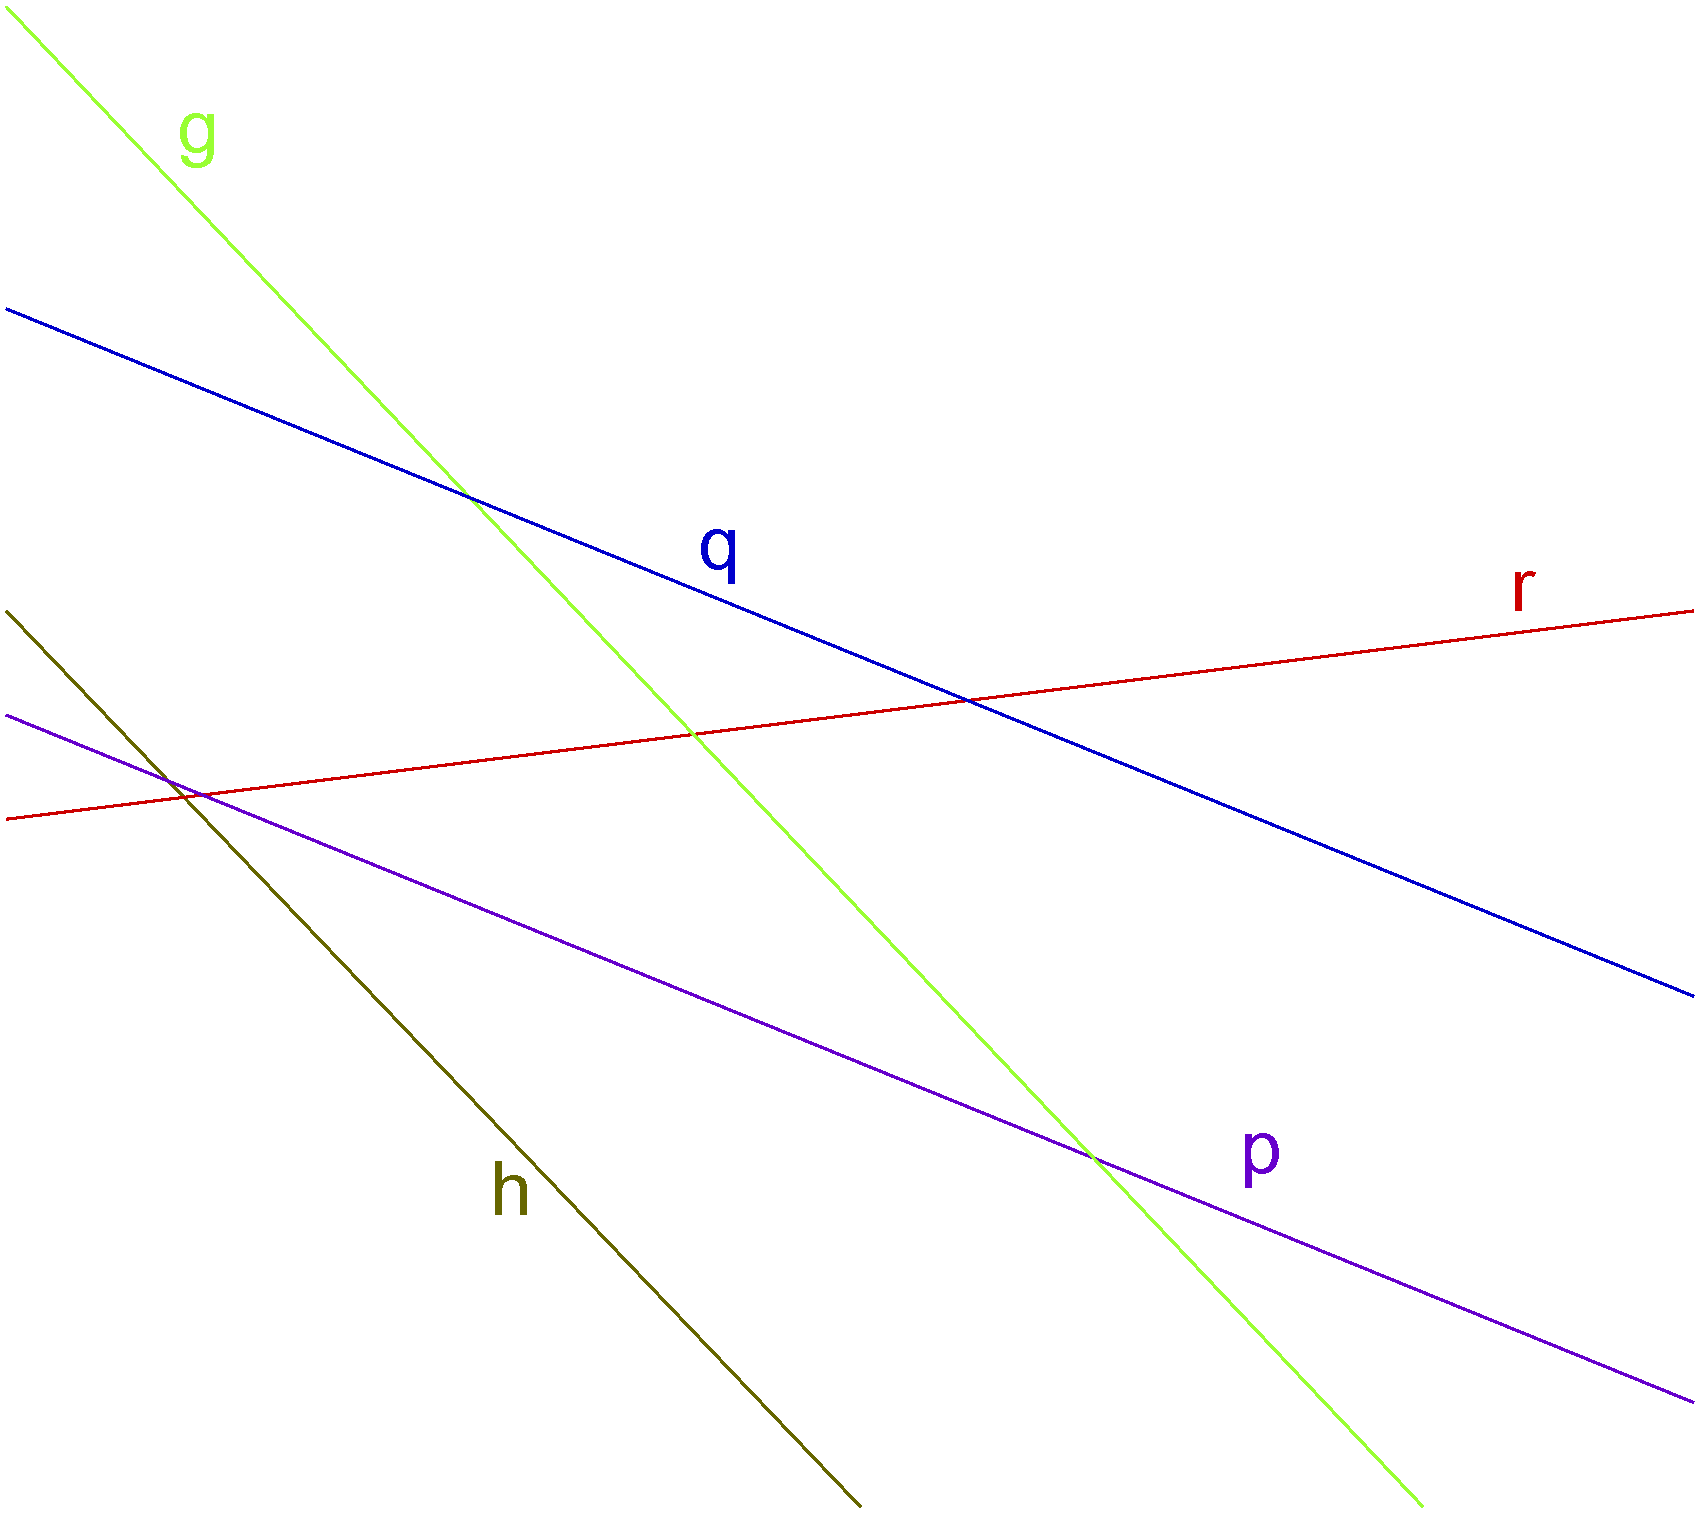
\includegraphics[width=0.5\textwidth]{figures/geraden}
    %\end{framed}
    \end{center}
    Offenbar gelten folgende Beziehungen:
    \begin{itemize}
    \item Die Gerade $g$ steht in Relation $R_1$ zu folgenden Geraden: $g$, $h$.
    \item Die Gerade $h$ steht in Relation $R_1$ zu folgenden Geraden: $g$, $h$.
    \item Die Gerade $p$ steht in Relation $R_1$ zu folgenden Geraden: $p$, $q$.
    \item Die Gerade $q$ steht in Relation $R_1$ zu folgenden Geraden: $p$, $q$.
    \item Die Gerade $r$ steht mit keiner anderen Geraden in Relation $R_1$.
    \end{itemize}
    Als Menge geschrieben, nimmt die Relation $R_1$ also folgende Gestalt an:
    \[
    R_1=\big\{(g,g),(g,h),(h,h),(h,g),(p,p),(p,q),(q,q),(q,p),(r,r)\big\}.
    \]
    Bildlich lässt sich die Relation als Tabelle darstellen:
    \begin{center}
    \begin{tabular}{ c | c c c c c }
    $r$&\xmark&\xmark&\xmark&\xmark&\cmark\\
    $q$&\xmark&\xmark&\cmark&\cmark&\xmark\\
    $p$&\xmark&\xmark&\cmark&\cmark&\xmark\\
    $h$&\cmark&\cmark&\xmark&\xmark&\xmark\\
    $g$&\cmark&\cmark&\xmark&\xmark&\xmark\\
    \hline
    &$g$&$h$&$p$&$q$&$r$
    \end{tabular}
    \end{center}
    Aus der Tabelle erhält man, ähnlich (gleich) wie im Fall von Funktionen und
    Funktionsgraphen, den Relationsgraph von $R_1$:
    \begin{center}
    \begin{tabular}{ c | c c c c c }
    $r$&&&&&\cellcolor{black}\\
    $q$&&&\cellcolor{black}&\cellcolor{black}&\\
    $p$&&&\cellcolor{black}&\cellcolor{black}&\\
    $h$&\cellcolor{black}&\cellcolor{black}&&&\\
    $g$&\cellcolor{black}&\cellcolor{black}&&&\\
    \hline
    &$g$&$h$&$p$&$q$&$r$
    \end{tabular}
    \end{center}
\end{example}
\end{comment}



\begin{definition}{Gerichteter Graph}
    Ein \textit{(gerichteter) Graph} ist ein Paar $G=(V,E)$ bestehend aus einer Menge $V$ (Knotenmenge)
    und einer binären Relation $E\subseteq V\times V$ (Kantenmenge).
\end{definition}






\subsection{Ordnungs- und Äquivalenzrelationen}

\begin{definition}{Eigenschaften von Relationen}
    Eine binäre Relation $R$ auf einer Menge $X$ heisst:
    \begin{itemize}
    \item \textit{Reflexiv}, wenn für alle $x\in X$
    \[
    xRx
    \]
    
    \item \textit{Symmetrisch}, wenn für alle $x,y\in X$
    \[
    xRy\,\Rightarrow\, yRx
    \]
    
    \item \textit{Antisymmetrisch}, wenn für alle $x,y\in X$
    \[
    xRy\land yRx\,\Rightarrow x=y
    \]
    
    \item \textit{Transitiv}, wenn für alle $x,y,z\in X$
    \[
    xRy\land yRz\,\Rightarrow \, xRz
    \]
    
    \end{itemize}
    \end{definition}




    \subsection*{Äquivalenzrelationen}

    Äquivalenzrelationen sind in einem gewissen Sinn verallgemeinerte Gleichheitsrelationen. Sie werden dazu verwendet, (im Sinn der Relation) ähnliche Objekte miteinander zu identifizieren und als ``gleich'' zu behandeln.

    \begin{definition}{Äquivalenzrelation}
    \textit{Äquivalenzrelationen} sind reflexive, symmetrische und transitive Relationen.
    \end{definition}


    \begin{definition}{Äquivalenzklasse}
    Es sei $R$ eine Äquivalenzrelation auf einer Menge $X$ und $x\in X$. Die \textit{Äquivalenzklasse} $[x]_R$ von $x$ bezüglich $R$ ist die Menge aller Elemente von $X$, die zu $x$ in Relation $R$ stehen:
    \[
    [x]_R:=\{y\in X\mid xRy \}
    \]
    Jedes Element einer Äquivalenzklasse nennen wir einen \textit{Repräsentanten} der entsprechenden Äquivalenzklasse. Die \textit{Faktormenge} $\faktor{X}{R}$ \textit{von} $X$ \textit{modulo} $R$ ist die Menge aller Äquivalenzklassen:
    \[
    \faktor{X}{R}:=\big\{ [x]_R\mid x\in X \big\}
    \]
    \end{definition}

    
    \begin{lemma}{Äquivalente Elemente}
    Ist $\sim $ eine Äquivalenzrelation auf einer Menge $X$ und gilt $x,y\in X$ mit $x\sim y$, dann gilt $[x]_\sim=[y]_\sim$. Mit anderen Worten, äquivalente Elemente repräsentieren stets dieselbe Äquivalenzklasse.
    \end{lemma}
    
    \begin{proof}{Äquivalenz zeigen}
    Seien $X,\sim,x,y$ wie in der Behauptung. Um zu zeigen, dass $[x]_\sim=[y]_\sim$ gilt, genügt es nachzuweisen, dass $x\sim z\Leftrightarrow y\sim z$ für beliebige $z\in X$ gilt. Wir nehmen $x\sim y$ an, dann gilt
    \begin{align*}
    y\sim z\Rightarrow x\sim y\land y\sim z \stackrel{\text{Transitivität}}{\Longrightarrow} x\sim z
    \end{align*}
    und
    \[
    x\sim z\Rightarrow x\sim y\land x\sim z\stackrel{\text{Symmetrie}}{\Longrightarrow} y\sim x\land x\sim z\stackrel{\text{Transitivität}}{\Longrightarrow} y\sim z,
    \]
    wie gewünscht.
    \end{proof}
    
    \begin{corollary}{Elemente als Repräsentanten}
    Ist $\sim $ eine Äquivalenzrelation auf $X$ und sind $x,y\in X$ mit $x\in[y]_\sim$, dann gilt $[x]_\sim=[y]_\sim$. Mit anderen Worten, jedes Element einer Äquivalenzklasse ist auch ein Repräsentant dieser Äquivalenzklasse.
    \end{corollary}
    
    \begin{proof}{Äquivalenz zeigen Variante 2}
    Es seien $X,\sim,x$ und $y$ wie in der Behauptung. Aus $x\in[y]_\sim$ folgt $y\sim x$. Die Behauptung folgt nun aus Lemma~\ref{lm:sim gleiche klasse}.
    \end{proof}

    \begin{lemma}{Disjunktheit Equivalenzklassen}
    Ist $\sim $ eine Äquivalenzrelation auf $X$ und sind $x,y\in X$ mit $[x]_\sim\neq[y]_\sim$, dann gilt $[x]_\sim\cap[y]_\sim=\varnothing$.
    Mit anderen Worten, verschiedene Äquivalenzklassen sind immer disjunkt.
    \end{lemma}
    
    \begin{proof}{Disjunktheit von Äquivalenzklassen zeigen}
    Es seien $X,\sim,x$ und $y$ wie in der Behauptung. Wir zeigen die Kontraposition, d.h.
    \[
    [x]_\sim\cap[y]_\sim\neq\varnothing\Rightarrow [x]_\sim=[y]_\sim.
    \]
    Es gelte also $[x]_\sim\cap[y]_\sim\neq\varnothing$, es gibt daher ein $z\in [x]_\sim\cap[y]_\sim$. Daraus folgt, dass $x\sim z\land y\sim z$ gilt und wegen der Transitivität und der Symmetrie von $\sim$ folgt sofort $x\sim y$. Die Behauptung folgt nun aus Lemma~\ref{lm:sim gleiche klasse}.
    \end{proof}


    \begin{lemma}{Equivalenzklassen Partition}
    Ist $\sim$ eine Äquivalenzrelation auf einer Menge $X$, dann ist die Faktormenge $\faktor{X}{\sim}$ eine Partition von $X$.
    \end{lemma}
    
    \begin{proof}{Eigenschaften von Äquivalenzrelationen beweisen}
    Es sei $\sim$ eine beliebige Äquivalenzrelation auf einer Menge $X$. Wir müssen folgende Punkte verifizieren:
    \begin{enumerate}
    \item\label{a} Die Äquivalenzklassen sind alle nichtleer.
    \item\label{2} Die Äquivalenzklassen sind paarweise disjunkt.
    \item\label{3} Es gilt
    \[
    \bigcup_{x\in X}[x]_{\sim}=X.
    \]
    \end{enumerate}
    Der erste Punkt folgt aus der Definition von der Faktormenge (die Äquivalenzklassen sind via ihrer Repräsentanten definiert). Die Tatsache, dass die Äquivalenzklassen paarweise disjunkt sind, ist genau die Aussage von dem Satz Disjunktheit von Äquivalenzklassen. Wir brauchen also bloss noch den letzten Punkt zu verifizieren. Dies folgt, da für jedes $z\in X$, wegen der Reflexivität, $z\sim z$ und somit
    \[
    z\in[z]_\sim\subseteq\bigcup_{x\in X}[x]_\sim
    \]
    gilt.
    \end{proof}



    \begin{lemma}{Partition induziert Äquivalenzrelation}
    Ist $P=\{A_i\mid i\in I\}$ eine Partition von der Menge $X$, dann ist die Relation $\sim$, gegeben durch
    \[
    x\sim y:\Leftrightarrow \exists i\in I\,(x\in A_i\land y\in A_i),
    \]
    eine Äquivalenzrelation auf $X$. Zusätzlich gilt
    \[
    \faktor{X}{\sim}=P.
    \]
    \end{lemma}
    
    \begin{proof}{Äquivalenzrelation verifizieren}
    Zuerst zeigen wir, dass die Relation $\sim$ unter den gegebenen Umständen eine Äquivalenzrelation ist.
    \begin{itemize}
    \item \textbf{Reflexivität}: Sei $x\in X$  beliebig. Wir müssen zeigen, dass $x\sim x$ gilt. Da $P=\{A_i\mid i\in I\}$ eine Partition von $X$ ist, gibt es ein $i\in I$ mit $x\in A_i$, daraus folgt sofort $x\sim x$.
    \item \textbf{Symmetrie}: Es gelte $x\sim y$. Wir müssen $y\sim x$ zeigen. Aus $x\sim y$ folgt, dass es ein $i\in I$ mit $x\in A_i\land y\in A_i$ gibt, dies ist offensichtlich äquivalent zu $y\sim x$.
    \item \textbf{Transitivität}: Es gelte $x\sim y\land y\sim z$. Wir müssen $x\sim z$ zeigen. Aus $x\sim y\land y\sim z$ folgt, dass es $i,j\in I$ gibt so, dass $x,y\in A_i$ und $y,z\in A_j$ gilt. Da $P=\{A_i\mid i\in I\}$ eine Partition ist, kann $y $ nicht in zwei verschiedenen Blöcken enthalten sein, es gilt daher $i=j$ und somit $x\sim z$.
    \end{itemize}
    Dass die Äquivalenzklassen von $\sim$ genau den Blöcken von $P$ entsprechen ist sofort klar, wenn man beachtet, dass zwei Elemente genau dann äquivalent sind, wenn sie im selben Block von $P$ liegen.
    \end{proof}

    \begin{lemma}{Äquivalenzrelationen: Verallgemeinerte Gleichheit}
    Für jede Relation $\sim$ auf einer Menge $X$ sind folgende beiden Aussagen äquivalent.
    \begin{enumerate}
    \item[1.] Die Relation $\sim$ ist eine Äquivalenzrelation.
    \item[2.] Es gibt eine Menge $Y$ und ein Funktion $F:X\to Y$ so, dass für alle $x,y\in X$
    \[
    x\sim y\Leftrightarrow F(x)=F(y)
    \]
    gilt.
    \end{enumerate}
    \end{lemma}
    
    \begin{proof}{Gleichheit in Äquivalenzrelationen zeigen}
    Wenn $\sim$ eine Äquivalenzrelation auf der Menge $X$ ist, dann erfüllt die Abbildung
    \[
    F:X\to\mathcal{P}(X)\phantom{abstand}\text{mit} \phantom{abstand} F(x)=[x]_\sim
    \]
    alle geforderten Eigenschaften. Ist umgekehrt eine Funktion $F:X\to Y$ wie in der Behauptung gegeben, dann gilt für die Relation $\sim$ Folgendes:
    \begin{itemize}
    \item\textbf{Reflexivität} gilt, da für jedes Element $x\in X$ trivialerweise $F(x)=F(x)$ gilt.
    \item \textbf{Symmetrie} folgt, da für beliebige Elemente $x,y\in X$
    \[
    x\sim y\Rightarrow F(x)=F(y)\Rightarrow F(y)=F(x)\Rightarrow y\sim x
    \]
    gilt.
    \item\textbf{Transitivität} folgt, da für beliebige Elemente $x,y,z\in X$
    \[
    x\sim y\land y\sim z\Rightarrow F(x)=F(y)\land F(y)=F(z)\Rightarrow F(x)=F(z)\Rightarrow  x\sim z
    \]
    gilt.
    \end{itemize}
    \end{proof}


    \subsection*{Ordnungsrelationen}

    \begin{definition}{Minimale Elemente}
    Es sei $R$ eine binäre Relation auf der Menge $M$.
    \begin{itemize}
    \item Zwei Elemente $x,y\in M$ heissen $R$-\textit{unvergleichbar}, falls weder $xRy$ noch $yRx$ gilt.
    \item Ein Element $x\in X$ einer Teilmenge $X\subseteq M$ von $M$ heisst $R$-\textit{minimal in $X$}, falls es kein anderes Element $y\in X$ mit $yRx$ gibt.
    \item  Ein Element $x\in X$ einer Teilmenge $X\subseteq M$ von $M$ heisst $R$-\textit{maximal in $X$}, falls es kein anderes Element $y\in X$ mit $xRy$ gibt.
    \end{itemize}
    Wenn keine Missverständnisse zu befürchten sind, dann schreiben wir anstelle von $R$-minimal, $R$-maximal und $R$-unvergleichbar auch einfach minimal, maximal und unvergleichbar.
    \end{definition}


    \begin{definition}{Ordnungsrelation}
    Es sei $R$ eine binäre Relation auf der Menge $M$.
    \begin{itemize}
    \item $R$ ist eine \textit{Präordnung} auf $M$, wenn $R$ reflexiv und transitiv ist.
    \item $R$ ist eine \textit{Halbordnung} auf $M$, wenn $R$ reflexiv, antisymmetrisch und transitiv ist.
    \item $R$ ist eine \textit{totale oder lineare Ordnung} auf $M$, wenn $R$ eine Halbordnung ist und keine $R$-unvergleichbaren Elemente existieren.
    \item $R$ ist eine \textit{Wohlordnung} auf $M$, wenn $R$ eine totale Ordnung auf $M$ ist so, dass jede Teilmenge $X\neq\varnothing$ von $M$ (mindestens) ein $R$-minimales Element enthält.
    \end{itemize}
    \end{definition}


    \begin{example}~
    \begin{itemize}
    \item Die Relation $\leq$ auf der Menge $\R$ ist eine totale Ordnung, die aber keine Wohlordnung ist (die Menge $\{x\in\R\mid 0<x<1\}$ hat kein kleinstes Element). Auf der Menge $\N$ ist $\leq$ eine Wohlordnung\footnote{Ein Beweis dazu kommt im nächsten Kapitel.}. Auf der Menge $\Z$ ist die Relation $\leq$ keine Wohlordnung. Wieso?
    \item Ist $A$ eine Menge von Mengen, dann ist die Teilmengenrelation $\subseteq$ eine Halbordnung.
    \item Die Teilerrelation $T$ auf der Menge $\Z$ ist eine Halbordnung aber keine totale Ordnung. Die Elemente $7$ und $5$ sind $T$-unvergleichlich.
    \end{itemize}
    \end{example}

    \begin{definition}{Transitiver Abschluss}
        Es sei $R$ eine (bin\"are) Relation.
        \begin{itemize}
            \item Als \textit{transitiven Abschluss} von $R$ bezeichnet man die kleinste
            (bezüglich $\subseteq$) transitive Relation, die $R$ als Teilmenge enthält,
            sie wird mit $R^+$ notiert.
            \item Die kleinste Relation, die $R^+$ enthält und reflexiv ist, nennt man den
            \textit{reflexiv-transitiven Abschluss} von $R$, sie wird mit $R^*$ bezeichnet.
        \end{itemize}
    \end{definition}

    \begin{remark}
        F\"ur eine beliebige (bin\"are) Relation $R$ gilt genau dann $xR^*y$, wenn es
        eine endliche Folge $x=k_1,\dots,k_n=y$ gibt, so dass $k_iRk_{i+1}$ f\"ur alle
        Indices $i=1,\dots,n-1$ gilt. Es gilt also genau dann $xR^*y$, wenn es eine Folge von
        Elementen gibt, die mit $x$ beginnt, mit $y$ endet und deren Elemente alle der Reihe
        nach in Relation $R$ zueinander stehen. Ist $G=(V,E)$ ein Graph, dann bedeutet
        $xE^*y$, dass in $G$ ein Pfad von $x$ nach $y$ existiert.
    \end{remark}

    \begin{definition} {Pfad und Zyklus}
        Ein \textit{Weg} oder \textit{Pfad} in einem Graph $G=(V,E)$ ist eine endliche Folge
        $k_1,\dots,k_n\in V$ von Knoten, so dass $k_iEk_{i+1}$ f\"ur alle Indices
        $i=1,\dots,n-1$ gilt. Die Knoten $k_1$ und $k_n$ bezeichnet man als \textit{Anfangs-}
        und \textit{Endpunkt} des Pfades. Gilt zusätzlich $k_1=k_n$, dann spricht man von einem \textit{Zyklus}.
    \end{definition}


    \begin{definition}{Topologische Sortierung}
        Es sei $M$ eine endliche Menge und $G=(M,E)$ ein DAG. Eine lineare Ordnung $\preceq\subseteq M\times M$ ist eine \textit{topologische Sortierung} von $G$, wenn für alle $a,b\in M$
        \begin{align*}
        a E^* b  \Rightarrow a\preceq b
        \end{align*}
        gilt.
    \end{definition}

    \begin{lemma}{Topologische Sortierung DAG}
        Jeder endliche DAG besitzt (mindestens) eine topologische Sortierung.
    \end{lemma}
    
    \begin{proof}{Topologische Sortierung DAG}
        Wir bemerken zuerst, dass jeder endliche DAG $G=(V,E)$ minimale Elemente bezüglich der Relation $E$ besitzt (wieso?). Weiter bemerken wir, dass jeder DAG, von dem ein minimaler Knoten (zusammen mit den von diesem Knoten ausgehenden Pfeilen) entfernt wird, wieder ein DAG ist (entfernen von Knoten und Verbindungen kann keine neuen Zyklen erzeugen). Aus diesen Beobachtungen folgt, dass folgender Algorithmus eine topologische Sortierung für jeden endlichen DAG generiert:
        \begin{enumerate}
            \item Wenn $G=(V,E)$ nicht leer ist, dann wähle ein bezüglich $E$ minimales Element $x\in V$ (Wenn $V$ leer ist, terminiere).
            \item Wiederhole die erste Instruktion mit $G'=(V\setminus \{x\},\{(a,b)\in E\mid a\neq x \})$ (d.h. erstelle den DAG $G'$ durch Entfernen von $x$ aus $V$ und entfernen von allen von $x$ ausgehenden Kanten in $E$).
        \end{enumerate}
    Die Reihenfolge, mit der die Elemente entfernt werden, entspricht einer topologischen Sortierung.
    \end{proof}


    \begin{lemma}{Halbordnung DAG}
        Folgende Aussagen sind äquivalent:
        \begin{enumerate}
            \item $(V,E\setminus \Delta_V)$ ist ein DAG.
            \item $E^*$ ist eine Halbordnung auf $V$.
        \end{enumerate}
    \end{lemma}
    
    \begin{proof}{Halbordnung DAG}
        $a)\Rightarrow b)$: Es sei $(V,E)$ ein DAG. Weil $E^*$ nach Definition bereits
        reflexiv und transitiv ist, müssen wir bloss noch zeigen, dass $E^*$
        antisymmetrisch ist. Gilt $xE^*y$, $yE^*x$ und $x\neq y$, dann gibt es
        Pfade $x,a_1,\dots,a_n,y$ und $y,b_1,\dots,b_m,x$ in $(V,E\setminus \Delta_V)$ (eventuell ist das Entfernen von Wiederholungen nötig, vgl. Wandtafel) und daher auch
        einen Zyklus $x,a_1,\dots,a_n,y,b_1,\dots,b_m$. Die Behauptung folgt per
        Kontraposition.

        $b)\Rightarrow a)$: Wenn $E^*$ eine Halbordnung ist, dann existieren aufgrund der
        Antisymmetrie keine Zyklen mit mehr als einem Knoten in $(V,E)$, daher existieren in
        $(V,E\setminus\Delta_V)$ gar keine Zyklen (vgl. Bild Wandtafel).
    \end{proof}

    \begin{corollary}{Halbordnung - lineare Ordnung}
        Jede endliche Halbordnung kann zu einer linearen Ordnung erweitert werden. Formal, zu jeder Halbordnung $\preceq$ auf einer Menge $M$ gibt es eine lineare Ordnung $\ll$ auf $M$, so dass
        \begin{align*}
        a\preceq b \Rightarrow a\ll b
        \end{align*}
        gilt.
    \end{corollary}
    
    \begin{proof}{Halbordnung - lineare Ordnung}
        Wir haben bereits gesehen, dass der Graph $G=(M,\preceq\setminus\Delta_M)$ ein DAG ist. Jede topologische Sortierung von $G$ erfüllt die Behauptung.
    \end{proof}


    \begin{lemma}{Wohlordnung - kleinstes Element}
    Ist $\preceq$ eine Wohlordnung auf einer Menge $M$, dann gibt es keine unendlich absteigende Folge
    \[
    a_0\succeq a_1\succeq\dots\succeq a_n\succeq a_{n+1}\succeq\dots
    \]
    von verschiedenen Elementen aus $M$.
    \end{lemma}
    
    \begin{proof}{Wohlordnung - kleinstes Element}
    Gibt es eine absteigende Folge $a_0,a_1,\dots$ wie in der Behauptung, dann ist die Menge
    \[
    \{a_i\mid i\in M\}
    \]
    eine Teilmenge von $M$, die kein $\preceq$-minimales Element besitzt. Die Relation $\preceq$ kann also in diesem Fall keine Wohlordnung sein. Die Behauptung folgt durch Kontraposition.
    \end{proof}


    \begin{example}
        Geben Sie zwei $\leq^*$ unvergleichbare Funktionen $f$ und $g$ an.
        \tcblower
        Zum Beispiel
            \begin{align*}
                f(n) =  \begin{cases}
                            1&\text{ falls $n$ gerade}\\
                            0&\text{ sonst}
                        \end{cases}
            \end{align*}
            und
            \begin{align*}
                g(n) =  \begin{cases}
                            0&\text{ falls $n$ ungerade}\\
                            1&\text{ sonst}
                        \end{cases}
            \end{align*}
    \end{example}

    \begin{definition}{Hasse-Diagramm}
    Es sei $\preceq$ eine Halbordnung auf einer Menge $M$. Das \textit{Hasse-Diagramm} von $R$ ist eine vereinfachte Darstellung des Graphen $(M,\preceq)$.
    \begin{itemize}
    \item Die Richtung eines Pfeiles $a\to b$ für Elemente $a,b\in M$ wird dadurch zum Ausdruck gebracht, dass sich der Knoten $b$ oberhalb von $a$ befindet.
    \item Pfeile zwischen zwei Punkten $a,b$ werden gelöscht, wenn es einen weiteren Punkt $c$ mit $a\preceq c\preceq b$ gibt.
    \item Pfeile, die von einem Punkt auf denselben Punkt zeigen (Schleifen), werden weggelassen.
    \end{itemize}
    \end{definition}

  